\section {Marco teórico y estado del arte}\label{sec:marco}
\subsection {Bases de datos y álgebra relacional}\label{subsec:rdb}
El \emph{modelo relacional de base de datos}, consiste en cinco componentes:
\begin{enumerate}
	\item Una colección de tipos escalares, pueden ser definidos por el sistema o por el usuario.
	\item Un generador de tipos de relaciones y un intérprete para las relaciones mismas.
	\item Estructuras para definir variables relacionales de los tipos generados.
	\item Un operador para asignar valores de relación a dichas variables.
	\item Una colección relacionalmente completa para obtener valores relacionales de otros valores relacionales mediante operadores.
\end{enumerate}
%Aunque tersa esta lista es útil para delimitar lo que el modelo relacional es y no es.
%Se debe comenzar definiendo los \emph{tipos}, ya que las relaciones se definen sobre ellos, \citeauthor{date12} (\citeyear{date12}) las define como
%\begin{displayquote}
%en esencia un conjunto finito de valores nombrados\textemdash todos los valores posibles de alguna categoría específica
%\end{displayquote}
%Los \emph{atributos} son pares ordenados de combinaciones atributo-nombre/tipo-nombre y una \emph{tupla} es un par ordenado de atributos.
%El modelo relacional también soporta varios tipos de \emph{llaves}, que poseen las propiedades de unicidad, ninguna contiene dos tuplas distintas con el mismo valor e irreductibilidad, ningún subconjunto suyo es tiene unicidad.
%%La llave foránea (\emph{FK}) es una combinación o set se atributos FK en una relación $r2$ tal que se requiere que cada valor FK sea igual a algún valor de alguna llave K en alguna relación $r1$ ($r1$ y $r2$ no son necesariamente distintos).
%\begin{table}[H]\centering\begin{tabular}{rc|c|c|l}
%		\cline{2-4}
%		\multicolumn{1}{r}{$\text{Atributos}\begin{cases}\ \end{cases}$}&\multicolumn{1}{|c|}{código}&\multicolumn{1}{c|}{fecha}&\multicolumn{1}{c|}{estado}&\multicolumn{1}{l}{}\\
%		\cline{2-4}
%		\multirow{3}{*}{$\text{Tuplas}\begin{cases}\\\\\end{cases}$}&\multicolumn{1}{|c|}{MX01}& 29-07-99&1&\multicolumn{1}{ l }{}\\
%		\cline{2-4}
%		&\multicolumn{1}{|c|}{MX02}&30-07-99&1&\multicolumn{1}{ l }{}\\
%		\cline{2-4}
%		&\multicolumn{1}{|c|}{MX03}&31-07-99&0&\multicolumn{1}{ l }{}\\
%		\cline{2-4}
%	\end{tabular}\caption{Representación de una tabla de una base en datos, la fila superior muestra tres atributos distintos y \emph{cada una} de las filas siguientes es una tupla.}\label{table:tupla}\end{table}
%La \emph{restricción de integridad} (\emph{constraint}) es una expresión booleana que debe evaluarse como verdadera. Los \emph{constraints de tipo} definen los valores que constituyen un tipo dado y los \emph{constraints de base de datos} limitan los valores que pueden aparecer en cierta base de datos. Las bases de datos suelen tener múltiples constraints específicos, expresados en términos de sus relaciones, sin embargo, el modelo relacional incluye dos constraints genéricos, que aplican a cada base de datos:
%\begin{itemize}
%	\item Regla de integridad de identidad: Las \emph{llaves primarias} (\emph{PK}) deben ser no nulas.
%	\item Regla de integridad de referencia: Las \emph{llaves foráneas} (\emph{FK}) deben tener relación (si $B$ referencia a $A$, $A$ debe existir).
%\end{itemize}
Las operaciones del modelo relacional están cimientadas en el \emph{álgebra relacional}.
%\begin{displayquote}
%	en esencia un conjunto finito de valores nombrados\textemdash todos los valores posibles de alguna categoría específica(\citeauthor{date12}, \citeyear{date12})
%\end{displayquote}
Utilizando operaciones primitivas del álgebra se producen nuevas relaciones que pueden manipularse también por medio de operaciones del álgebra mismo. Una secuencia de operaciones de álgebra relacional forma una expresión cuyo resultado es una relación que representa el resultado de una consulta de base de datos. Estas operaciones se pueden clasificar en dos grupos, operaciones de la teoría de conjuntos: \emph{UNIÓN}, \emph{INTERSECCIÓN}, \emph{DIFERENCIA} y \emph{PRODUCTO CARTESIANO} (\emph{PRODUCTO CRUZADO}), y el otro grupo consiste en operaciones específicas para bases de datos relacionales: \emph{JUNTAR}, \emph{SELECCIONAR} y \emph{PROYECTAR}.
% Estas dos últimas, por operar con una sola relación, son también conocidas como \emph{operaciones unarias}.

% SELECCIONAR elige un subconjunto de tuplas de una relación que satisfacen la condición de selección
% \begin{equation}
% \sigma_\text{\textless condición de selección\textgreater}{\text{(R)}}
% \end{equation}
% donde $\sigma$ denota el operador SELECCIONAR, y la condición de selección es una expresión booleana especificada en los atributos de la relación $R$.

% PROYECTAR produce una nueva relación de atributos y tuplas duplicadas
% \begin{equation}
% \pi_\text{\textless lista de atributos\textgreater}{\text{(R)}}
% \end{equation}
% donde $\pi$ es el denota el operador PROYECTAR y la lista de atributos es la sublista de atributos deseados de la relación $R$.

% Las operaciones con dos relaciones reciben el nombre de \emph{operaciones binarias}. Si las relaciones $R(A_1,A_2,\ldots,A_n)$ y $S(B_1,B_2,\ldots,B_n)$ son \emph{compatibles con la unión} (tienen el mismo grado $n$ y $dom(A_i)=dom(B_i)$ para $1\leq i\leq n$) podemos usarlas para definir las siguientes operaciones binarias:
% \begin{itemize}
% 	\item UNIÓN: El resultado de esta operación se denota $R \cup S$, es una relación que incluye todas las tuplas que están en $R$, $S$ o ambos, se eliminan duplicados.
% 	\item INTERSECCIÓN: El resultado de esta operación se denota $R \cap S$, es una relación que incluye todas las tuplas que están en ambos $R$ y $S$.
% 	\item DIFERENCIA: El resultado de esta operación se denota $R - S$, es una relación que incluye todas las tuplas que están en ambos $R$ pero no en $S$.
% \end{itemize}

% PRODUCTO CARTESIANO denotado $R \times S$ es la operación binaria que no requiere compatibilidad con la unión y produce un nuevo elemento al combinar cada miembro (tupla) de cada relación con cada otro miembro de la otra relación. El resultado de $R(A_1,A_2,\ldots,A_n)$ y $S(B_1,B_2,\ldots,B_m)$ es una relación $Q$ con atributos $Q(A_1,A_2,\ldots,A_n,B_1,B_2,\ldots,B_m)$ (en ese orden) de grado $n+m$. El resultado $Q$ tiene una tupla por cada combinación de tuplas de $R$ y $S$.

% JUNTAR $\Join$, es el operador utilizado para combinar tuplas relacionadas de dos relaciones en una sola tupla. Pertinente para procesar relaciones entre relaciones. Si tenemos dos relaciones $R(A_1,A_2,\ldots,A_n)$ y $S(B_1,B_2,\ldots,B_m)$ podemos escribir la operación JUNTAR como
% \begin{equation}
% R\Join_\text{\textless condiciones de unión\textgreater}S,
% \end{equation}
% el resultado es la relación $Q$ con atributos $Q(A_1,A_2,\ldots,A_n,B_1,B_2,\ldots,B_m)$ (en ese orden). El resultado $Q$ tiene una tupla por cada combinación de tuplas de $R$ y $S$ que satisfacen las condiciones de unión.
\begin{wrapfigure}{h}{4.4cm}
	\begin{tikzpicture}
	\def\IA{(0,0) circle (1.6cm)}
	\def\AM{(270:.666cm) circle (1cm)}
	\def\AP{(270:1.33cm) circle (.666cm)}
	\draw \IA node[above]{\tiny $^{^{^{^{\overset{\text{Inteligencia artificial}}{}}}}}$};
	\draw \AM node[above]{\tiny $^{^{^{\overunderset{\text{Aprendizaje}}{\text{maquinal}}{}}}}$};
	\draw \AP node{\tiny $\overunderset{\text{Aprendizaje}}{\text{profundo}}{}$};
	\end{tikzpicture}\caption[Inteligencia Artificial]{\tiny Aprendizaje profundo, es un subcampo del aprendizaje maquinal, que a su vez es un subcampo de la inteligencia artificial}\end{wrapfigure}\label{fig:AI}